\section{Introduction}\label{sec:introduction}
%Describe motivation of the problem (navigation is important for robots)
One of the most important tasks that humans perform in their daily lives is semantic and goal-oriented navigation.
This ability to navigate like a human towards a target in the environment is considered one of the ``holy grail'' goals of intelligent robots.
There are countless applications that could be supported by a robotic platform with this capacity.
From assistive robots that can accompany a person to perform a specific task, to platforms that navigate autonomously in complex work environments, such as logistics centers.

%Describe the problem of visual semantic navigation (briefly)
In this work, we address the problem of visual semantic navigation (VSN).
%In other words, mainly using vision-based sensors, we want a robot to learn to navigate through an environment so that it is able to reach a particular object in the surroundings, \eg a chair.
The goal is to make a robot capable of navigating through an environment to reach a particular object (the target) in the surroundings, such as a chair, mainly using vision-based sensors.
Technically, a VSN approach is a learning-based navigation model, where no geometry-based traditional techniques are applied.
Nor the map of the environment is known a priori, neither the map is built on the fly.
The majority of methods integrate reinforcement learning (RL) techniques with current developments in deep learning models for visual perception.

\begin{figure}[t]
  \centering
   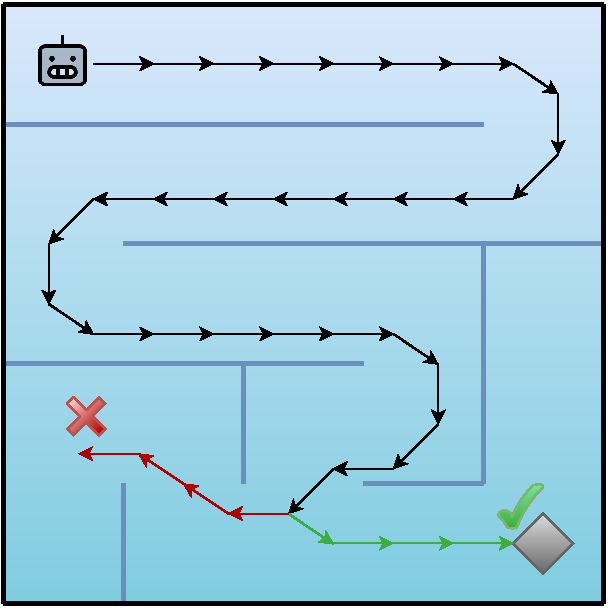
\includegraphics[width=0.6\linewidth]{graphics/graphical_abstract}
   \caption{Can an agent pinpoint a target in a maze using a visual semantic navigation (VSN) model based on state-of-the-art RL and deep learning models? We explore and analyze the solutions for the main challenges in VSN, \ie unknown environments, visibility of targets and path planning.} 
   \label{fig:graphical_abstract}
\end{figure}

%Describe the problem we address (use the graphical abstract)
The main questions we want to address in this work are: Is it possible to offer accurate experimental evaluation settings so that different RL-based VSN models may be clearly compared to one another?; What are the main challenges associated to these RL-based VSN models?
With respect to the former, after reviewing the literature, we come to the conclusion that it is difficult to make direct comparisons between the many solutions provided.
The key challenges are that the navigation settings in which the experimental metrics are given are not available, and that each technique employs a separate set of RL libraries.
With respect to the second question, three are the main challenges that every VSN model needs to tackle.
See Figure~\ref{fig:graphical_abstract}.

Is it possible for an agent to localize a target in a maze with a VSN model based on state-of-the-art deep learning and RL models?
To begin with, it must be taken into consideration that the environment is, or might be, unknown to the agent.
In our experiments, we expose our agent to different mazes.
In this situation, the robot would need to explore the environment to learn more about it.
Second, how does the agent deal with the visibility of the targets?
For a VSN model, the object we have to navigate to may not be visible at the beginning or during navigation.
How does the agent learn a search strategy to find the object in the maze?
And third, even if the target is visible, the robot must devise a feasible route to reach it.



%Highlight our contributions
The main contributions of our work are as follows: 
\begin{enumerate}
 \item We propose a VSN model which leverages state-of-the-art Contrastive Language Image Pretraining (CLIP) encoders~\cite{radford2021}.
Technically, we have designed a model that combines a CLIP encoder with a set of two recurrent neural networks for producing the discrete navigation actions that our agent needs to take (Section~\ref{sec:navigation}).
  \item The agent is trained following a RL paradigm for VSN. We propose to evaluate the impact of each of the VSN challenges mentioned above, using different techniques that have been proposed in the literature: reward shaping~\cite{sutton2018, wijmans2020} to deal with the sparsity of the reward signal naturally associated to the navigation problem; and $\epsilon\text{-}greedy$~\cite{mnih2013} as a mechanism to balance exploitation and exploration.
  \item We have designed a thorough experimental evaluation setup (Section~\ref{sec:experiments}) with which we aim to offer a clear experimental environment in which to compare different VSN approaches.
 It has been implemented using pyRIL~\cite{pyRIL}, an open source python library for RL, and two navigation environments: a maze navigation setup of Miniwolrd-Maze from \textit{gym-miniworld}~\cite{gym_miniworld}; and a navigation through a 3D photorealistic scan indoor space provided by HM3D dataset~\cite{ramakrishnan2021} in Habitat~\cite{szot2021} simulator. 
 We release the codes to reproduce our experiments, as well as the whole experimental setup, so that others can compare their work with our results.
\end{enumerate}